\documentclass[border=4pt]{standalone}

\usepackage{amsmath}
\usepackage{tikz}
\usepackage{mathdots}
\usepackage{yhmath}
\usepackage{cancel}
\usepackage{color}
\usepackage{siunitx}
\usepackage{array}
\usepackage{multirow}
\usepackage{amssymb}
\usepackage{gensymb}
\usepackage{tabularx}
\usepackage{booktabs}
\usetikzlibrary{fadings}
\usetikzlibrary{patterns}


\begin{document}
 



\tikzset{every picture/.style={line width=0.75pt}} %set default line width to 0.75pt        

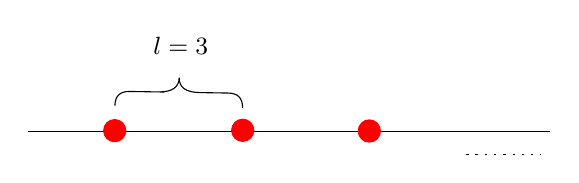
\begin{tikzpicture}[x=0.75pt,y=0.75pt,yscale=-1,xscale=1]
%uncomment if require: \path (0,300); %set diagram left start at 0, and has height of 300

%Straight Lines [id:da42589445731204423] 
\draw    (118,138) -- (369.5,138) ;


%Shape: Circle [id:dp03729110178660555] 
\draw  [color={rgb, 255:red, 255; green, 0; blue, 0 }  ,draw opacity=1 ][fill={rgb, 255:red, 255; green, 0; blue, 0 }  ,fill opacity=1 ] (154.33,137.5) .. controls (154.33,134.55) and (156.72,132.17) .. (159.67,132.17) .. controls (162.61,132.17) and (165,134.55) .. (165,137.5) .. controls (165,140.45) and (162.61,142.83) .. (159.67,142.83) .. controls (156.72,142.83) and (154.33,140.45) .. (154.33,137.5) -- cycle ;
%Shape: Circle [id:dp35342355415598425] 
\draw  [color={rgb, 255:red, 255; green, 0; blue, 0 }  ,draw opacity=1 ][fill={rgb, 255:red, 255; green, 0; blue, 0 }  ,fill opacity=1 ] (216,137.33) .. controls (216,134.39) and (218.39,132) .. (221.33,132) .. controls (224.28,132) and (226.67,134.39) .. (226.67,137.33) .. controls (226.67,140.28) and (224.28,142.67) .. (221.33,142.67) .. controls (218.39,142.67) and (216,140.28) .. (216,137.33) -- cycle ;
%Shape: Circle [id:dp4495579741387976] 
\draw  [color={rgb, 255:red, 255; green, 0; blue, 0 }  ,draw opacity=1 ][fill={rgb, 255:red, 255; green, 0; blue, 0 }  ,fill opacity=1 ] (277,137.67) .. controls (277,134.72) and (279.39,132.33) .. (282.33,132.33) .. controls (285.28,132.33) and (287.67,134.72) .. (287.67,137.67) .. controls (287.67,140.61) and (285.28,143) .. (282.33,143) .. controls (279.39,143) and (277,140.61) .. (277,137.67) -- cycle ;
%Straight Lines [id:da3462284467757739] 
\draw  [dash pattern={on 0.84pt off 2.51pt}]  (329,149) -- (365,149) ;


%Shape: Brace [id:dp1399708255110006] 
\draw   (221.25,126.5) .. controls (221.32,121.83) and (219.03,119.46) .. (214.36,119.39) -- (200.61,119.16) .. controls (193.94,119.05) and (190.65,116.67) .. (190.73,112) .. controls (190.65,116.67) and (187.28,118.95) .. (180.61,118.84)(183.61,118.89) -- (166.86,118.62) .. controls (162.19,118.54) and (159.82,120.83) .. (159.75,125.5) ;

% Text Node
\draw (191.5,96.5) node  [font=\small]  {$l=3$};


\end{tikzpicture}
\end{document}
